\subsubsection{Pion Background}\label{section:star_background_pion}
The pion spectra are corrected for weak decays (mainly $K^0_S$ and $\Lambda^0$), muon contribution and background from the   detector dead-material interactions. The pion decay muons can be identified as pions due to the similar masses. These contributions are obtained from MC, where the true-level information is well known. Figure~\ref{fig:bkg_pion} shows the background contribution to the pion spectra as a function of $p_T$ in three ranges of $\xi$, separately for $\pi^-$ and $\pi^+$.  There were   negligible differences  observed between these  three ranges of $\xi$, since that the background contribution was averaged over $\xi$. The following parametrization was found to describe it:
\begin{equation}
f_{bkg}^{\pi}\left(p_T\right)=a_0\exp(a_1p_T)+a_2p_T^2+a_3p_T
\end{equation}
where $a_0-a_3$ are free paramaters of the fitted function.

The pion background contribution varies between $5\%$ at low-$p_T$  ($p_T=0.25$~GeV/c) and about $1\%$ at $p_T=1.0$~GeV/c for both negatively and positively charged pions.
\begin{figure}[htpb]
	\centering
	\begin{subfigure}{.49\textwidth}
		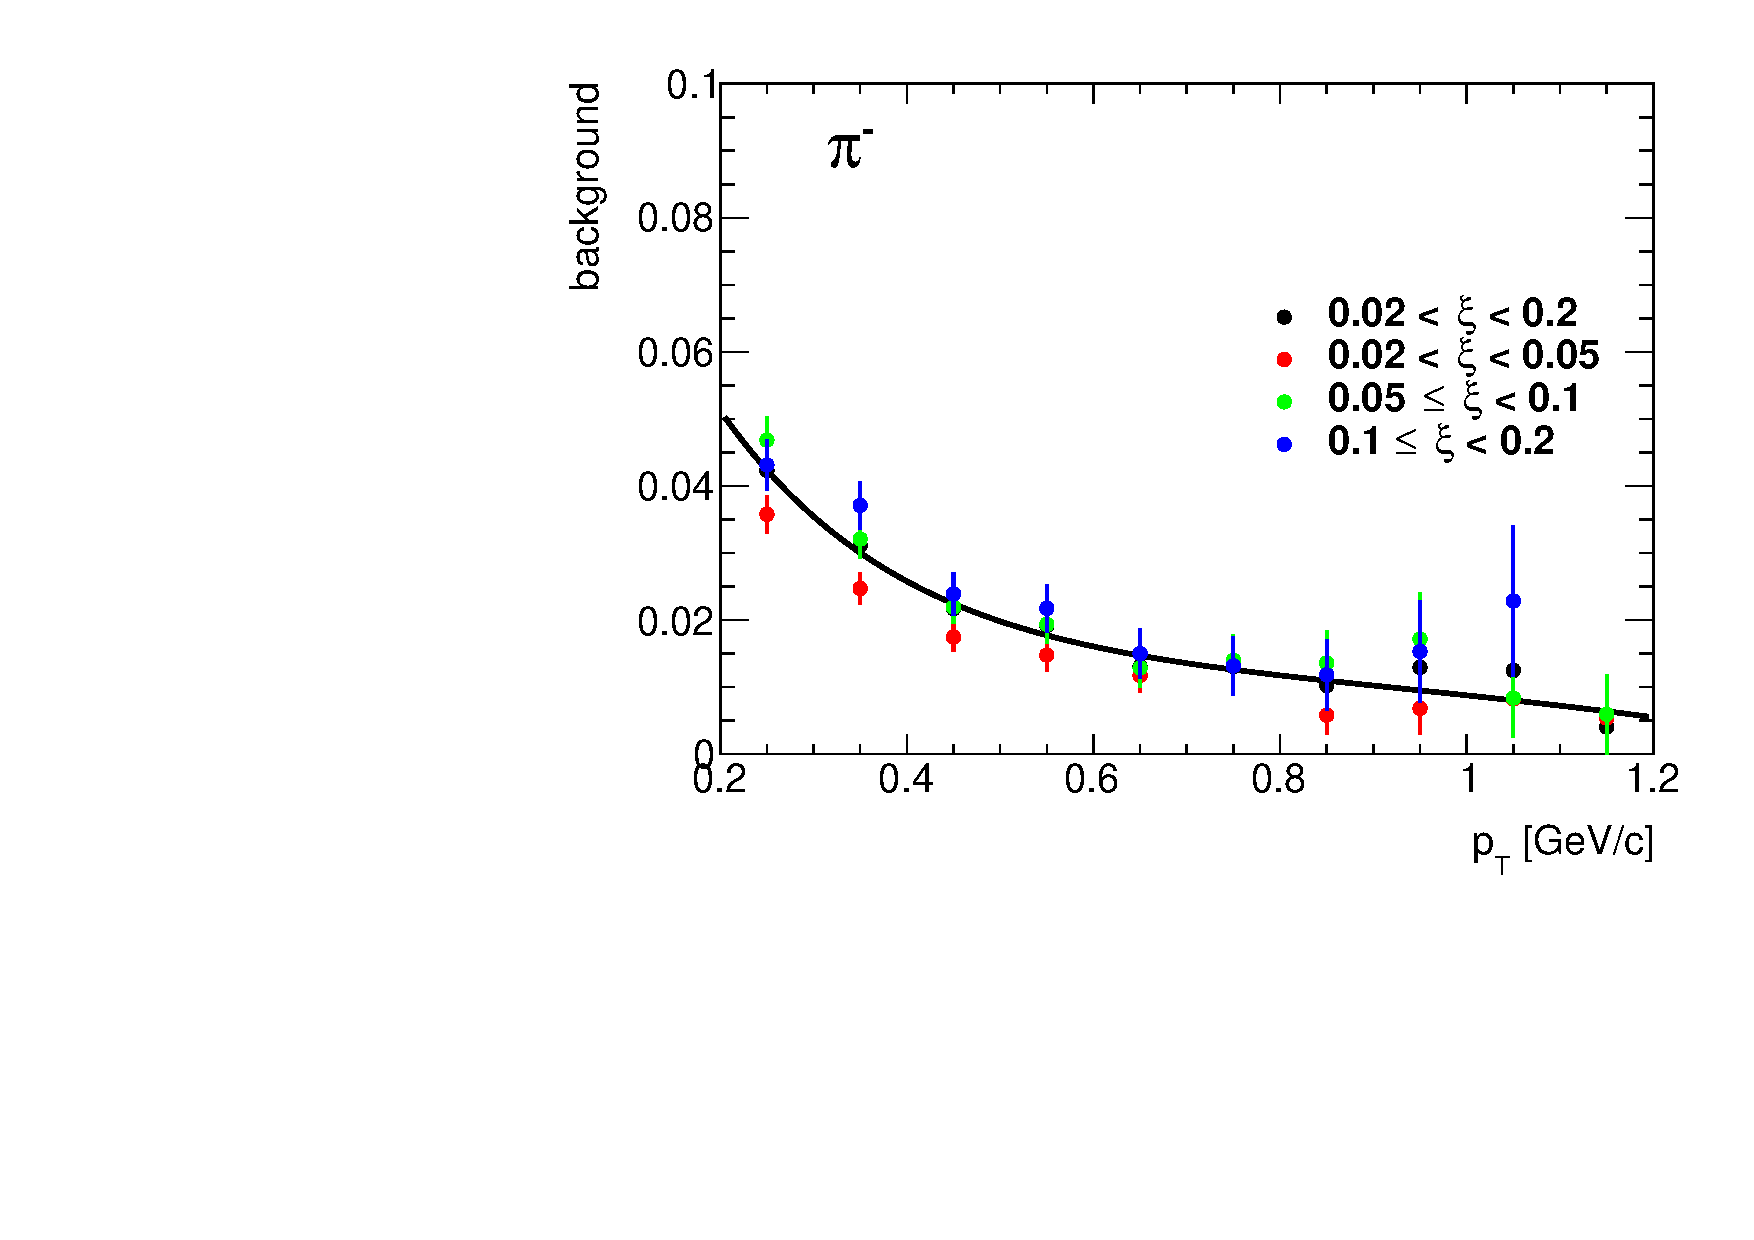
\includegraphics[width=\linewidth, page=1]{chapters/chrgSTAR/img/chargedBkg/bkg0max.pdf}
	\end{subfigure}
	\begin{subfigure}{.49\textwidth}
		\includegraphics[width=\linewidth, page=2]{chapters/chrgSTAR/img/chargedBkg/bkg0max.pdf}
	\end{subfigure}
	\caption[Pion background fraction as a function of $p_T$ shown separately for negatively (left)  and positively (right) charged pions in three ranges of $\xi$.]{Pion background fraction as a function of $p_T$ shown separately for negatively (left)  and positively (right) charged pions in three ranges of $\xi$: $0.02<\xi<0.05$ (red), $0.05<\xi<0.1$ (green), $0.1<\xi<0.2$ (blue). The pion background averaged over three ranges of $\xi$ with fitted parametrization is also shown (black). }
	\label{fig:bkg_pion}
\end{figure}

\FloatBarrier